\documentclass{article}
\usepackage[utf8]{inputenc}
\usepackage[spanish]{babel}

\title{Análisis del artículo “  Transformación  digital  e  innovación  educativa  en  Latinoamérica  en  el  marco  del COVID-19"}
\author{Rómulo Enrique Troncoso Pacheco}
\date{Noviembre 2020}

\usepackage{natbib}
\usepackage{graphicx}

\begin{document}

\maketitle

\section{Introducción}

En el presente trabajo de ingreso a la Maestría en Tecnología Informática Educativa, se compone de una serie de elementos que permiten identificar, analizar y aportar nuevas ideas relacionadas al artículo \citep{Ramirez} en estudio.
Para alcanzar dicho fin se desarrolló el trabajo mediante una seri de pasos sistemáticamente sugerido por la institución a evaluar donde se encuentra la fase de identificación de ideas principales las que se orientaron a un conjunto de siete ideas específicas que complementadas entre ellas, dan el resultado final del artículo. Además se completa con información adicional de otros autores que referencian teorías asociadas a la tecnología y su utilización en el campo educativo.
Seguidamente, se desarrolló aportes personales en base al artículo para una interpretación en fundamento a los datos ya obtenidos, mismas herramientas que fueron:
\begin{itemize}
    \item Programación en Python apoyado en la librería Matplotlib, encargada de la generación de las gráficas \citep{python}.
    \item Overleaf  utilizado como editor de texto online \citep{Overleaf} para la generación de un reporte en LaTeX \citep{latex}.
    \item GitHub como sistema de repositorio del trabajo, mismo que se encuentra en acceso público (romulotroncosop) \citep{Github}.
    \item Prezi utilizado como herramienta de presentación gráfica \citep{prezi}.
    \item Creately la que se utilizó como herramienta digital online para a creación de diagramas \citep{Creately}.
\end{itemize}
Una vez desarrollado lo anterior se procede a realizar los aportes personales del cómo se llevó a cabo en manera de redacción para finalizar con las conclusiones correspondientes orientadas al artículo y a las áreas temáticas designadas.



\section{Desarrollo}

\subsection{Ideas principales}
Al analizar el artículo referido por la institución evaluadora, se pudieron identificar las siguientes ideas, asimismo, se puede observar de manera gráfica en la Figura \ref{fig:diagrama}:
\subsubsection{Utilización de tecnologías en el proceso de enseñanza a aprendizaje}
\begin{enumerate}
    \item Necesidades emergentes.
    \item Entorno tecnológico.
    \item Co-evolución.
    \begin{itemize}
        \item Tecnología.
        \item Didáctica.
    \end{itemize}
\end{enumerate}
\subsubsection{Traspaso de aulas presenciales a aulas digitales}
\begin{enumerate}
    \item Modificaciones pedagógicas.
    \item Herramientas de aprendizaje.
\end{enumerate}
\subsubsection{Esencia de la transformación digital en las universidades}
\begin{enumerate}
    \item Tecnologías digitales para actividades.
    \item Cambios culturales.
    \item Cambios organizativos.
\end{enumerate}
\subsubsection{Tecnologías de la comunicación digital}
\begin{enumerate}
    \item Introducción de la enseñanza en red y a distancia.
    \item Desarrollo de servicios básicos de información.
    \item Creación e implementación del servicio de gestión en las universidades digitales.
\end{enumerate}
\subsubsection{Gestión del conocimiento}
\begin{enumerate}
    \item Transformación de la economía(física-digital).
    \item Producción.
    \item Educación.
    \item Capacidad de gestión.
    \item Flexibilidad.
    \item Formación del capital humano.
\end{enumerate}
\subsubsection{Innovación}
\begin{enumerate}
    \item Proceso.
    \begin{itemize}
        \item Educativo.
        \item Cognitivo.
    \end{itemize}
    \item Producto.
    \item Servicio.
    \item Conocimiento.
\end{enumerate}
\subsubsection{Desafíos}
\begin{enumerate}
    \item Gestión.
    \item Docencia.
    \item Cultura de innovación.
    \item Innovación tecnológica digital en procesos educativos.
    \item Innovación en procesos de investigación.
    \item Rediseño del enseñanza-aprendizaje en línea.
    \item Acervo tecnológico.
\end{enumerate}

\begin{figure}[ht]
    \centering
    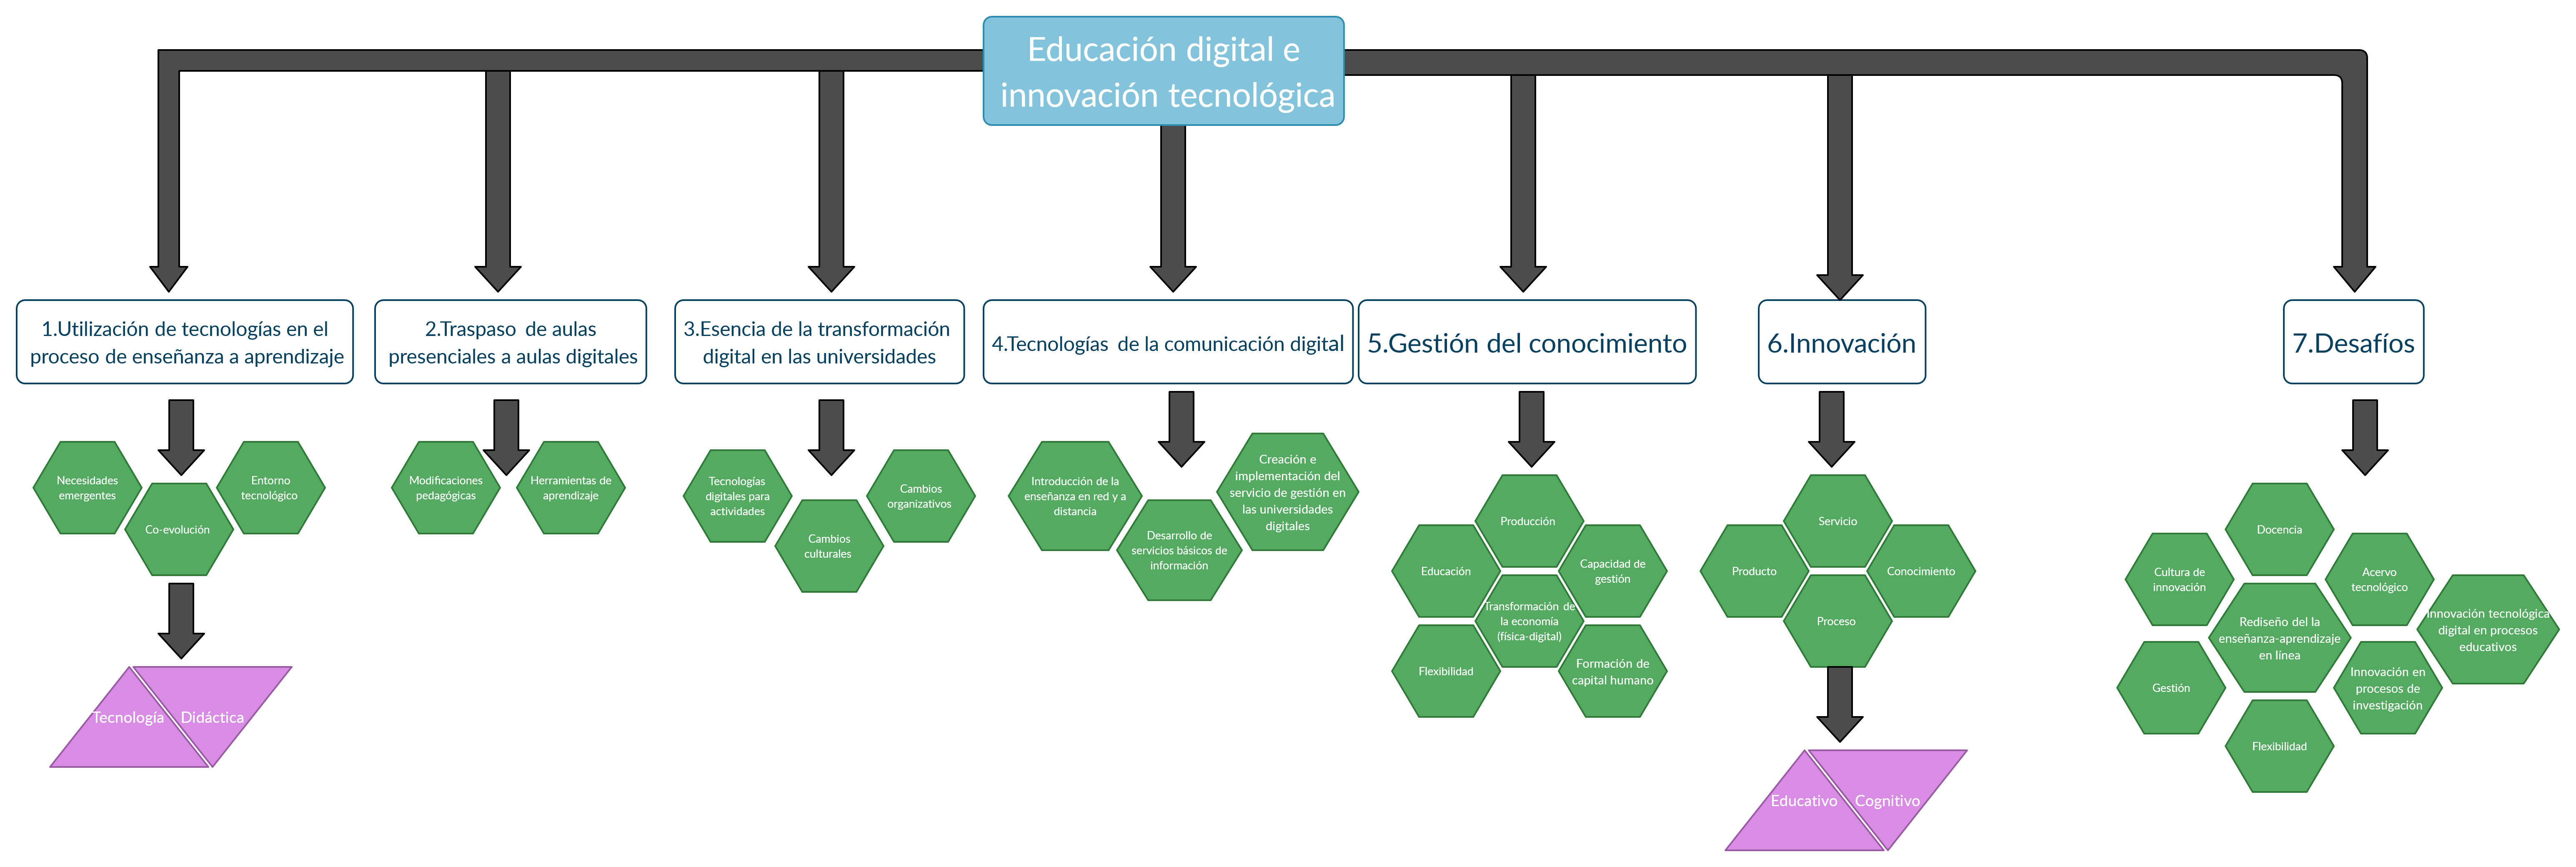
\includegraphics[scale=0.07]{diagrama.png}
    \caption{En las ideas principales en la presentación se puede observar con precisión por el tamaño deñ diagram, de igual manera se encontrara en el repositorio.}
    \label{fig:diagrama}
\end{figure}

\subsection{Desarrollo de ideas}
\subsubsection{Utilización de tecnologías en el proceso de enseñanza a aprendizaje}
Con la primera idea se pretende señalar la pertinencia que, de acuerdo a las necesidades inmediatas originadas por la pandemia a nivel internacional, fue necesario establecer nuevos escenarios de enseñanza y aprendizaje que permitieran llegar a los objetivos planeados en las asignaturas, orillando a los docentes a la implementación de nuevas tecnologías en un lapso de tiempo corto para el desarrollo de sus actividades académicas. 

\subsubsection{Traspaso de aulas presenciales a aulas digitales}
La contingencia sanitaria pudo dar evidencia de las necesidades inmediatas que se precisan en el proceso enseñanza aprendizaje para integrar métodos de formación del alumno como también de los procesos formativos  digitales del docente, en virtud que tuvieron que establecer nuevas técnicas de enseñanza mediante los recursos y herramientas tecnológicas, que, según el artículo revisado la gran mayoría de las universidades tuvieron que entrar a un proceso de capacitación para utilizar dichas herramientas.

\subsubsection{Esencia de la transformación digital en las universidades}
Las transformaciones referidas consisten de un modelo de 3.0 a uno de 4.0; lo que auxilia a una nueva implementación de tecnologías en las universidades, sin embargo, citado en el material, hace referencia a la imposibilidad por el acceso a tecnologías como también la falta de motivación por parte de los docentes al no querer implementar dichas herramientas tecnológicas por el desconocimiento. Mismos que ocasionan problemas de cultura y de cambios en la organización al realizar la transformación digital.

\subsubsection{Tecnologías de la comunicación digital}
Una de las primeras actividades de corte organizacional y de gestión por parte de las universidades fue el desarrollo de formación de competencias tecnológicas hacia los docentes, que auxiliaron a implementar herramientas básicas para el desarrollo de las aulas digitales. Asimismo, se tuvieron problemas de soporte técnico por la apresurada apertura de éstas, actualmente se les está brindando mantenimiento constante para evitar el fallo de la misma, lo que conlleva a una pérdida de tiempo en el desempeño académico.

\subsubsection{Gestión del conocimiento}
Para la autora la gestión del conocimiento lo integra como un punto de desarrollo estratégico para el avance digital, ya que en este punto se hace el señalamiento que se debe orientar a la producción con fundamento en la economía física a una digital; lo que conlleva un cambio en el sector educativo, las diversas estrategias para poder formar al capital humano, como también en la flexibilidad que los alumnos y docentes deben presentar en la conducta. 

\subsubsection{Innovación}
La autora plasma su idea de innovación enfocándose en varios puntos, establece un nuevo proceso con el fin de mejorar la organización, los métodos de aplicación, las estrategias como también el procedimiento, formación y técnica, mismos que impactarán directamente al funcionamiento educativo y cognitivo del estudiante; con el producto lo que se persigue es buscar nuevas herramientas que sirvan de base para un nuevo servicio a la población, y con esto establecido se pretende llegar a un nuevo conocimiento que está relacionado al proceso.

\subsubsection{Desafíos}
Los desafíos plasmados en el artículo fueron referenciados por las interrogantes descritas en la investigación, donde se puede identificar que para poder llegar a subsanar es importante la conjunción de esfuerzos entre la sociedad, sistema educativo/institucional, docentes, especialistas y alumnos; con el fin de poder rediseñar nuevas áreas de aprendizaje y poder dar una evolución de la educación tradicional a la educación digital.

\subsection{Aporte de otros autores}
\subsubsection{Utilización de tecnologías en el proceso de enseñanza a aprendizaje}
De esta manera el entorno tecnológico fue un recurso inmediato dentro del contexto educativo, en el cual se tuvo que soportar la enseñanza modificando las propias prácticas \citep{Barriaga} y cada uno de los modelos sugeridos por las asignaturas que obtienen mayor o menor complejidad en función de los grados y de los requerimientos a seguir en cada una de ellas.

\subsubsection{Traspaso de aulas presenciales a aulas digitales}
La migración de aulas presenciales hacia el aula digital, forzosamente es necesario reorganizar la metodología de la enseñanza que permitirá al docente y al alumno crear nuevas experiencias de aprendizaje; de esta manera, el docente debe integrar una serie de herramientas didácticas soportadas en los usos de la tecnología, todo ello, con la finalidad de poder concluir los objetivos de los materiales y siga permeando el interés de la currícula seleccionada, según sea cada disciplina \citep{Certificacion}.

\subsubsection{Esencia de la transformación digital en las universidades y cecnologías de la comunicación digital}
Las enseñanzas para ser llevadas a un plano digital, son necesarias una serie de nuevos desarrollos de planeación educativa, mismas que deben ser organizadas al mundo digital \citep{Modelos} para poder tener una pertinencia en el contexto educativo y poder brindar soluciones reales planteadas dentro de las necesidades emergente de la pandemia; por ello se necesita el cambio cultural de los actores educativos para poder ser partícipe de la enseñanza digital.
De esta manera el modelo 4.0, aborda el aprendizaje con la finalidad de solucionar problemas reales orientándose en las competencias \citep{Mapfre}, por ello el alumno, debe buscar estrategias para poder dar conclusión al problema establecido y de esta forma sea su propio motor de aprendizaje. De esta manera, las TICs son las herramientas tecnológicas que auxiliarán al alumno para facilitar el cumplimiento del objetivo pero NO es el objetivo.

\subsubsection{Gestión del conocimiento}
La gestión del conocimiento permite buscar nuevas estrategias de aprendizaje en el alumno y nuevas técnicas de enseñanza por parte del docente; por esta razón el crear ambientes apropiados mediatizados por las tecnologías permite accesar a la información y con el ello el desarrollo del conocimiento de los usuarios \citep{Botero}, permitiendo construir nuevos modelos de organización que impactarán a la sociedad moderna en lo referido a las organizaciones educativas como también en el tipo de formación de recurso humano de cada disciplina.

\subsubsection{Innovación}
Desde la perspectiva de la innovación educativa, debe ir a la par con la innovación y cambios en los medios sociales y culturales, ello permite que la innovación educativa no sea un fenómeno desarticulado con la realidad y que no cause rechazo en las prácticas de las aulas digitales. Por ello, implica una nueva forma de enseñar y también una nueva forma de aprender, de esta manera el rediseño del proceso de la enseñanza y aprendizaje debe ser pertinente en cada contexto evaluado. Por otro lado, existen áreas de impedimentos como lo son las oportunidades de acceso a la infraestructura adecuada que es uno de los grandes desafíos para generar conocimiento y la innovación en base al nuevo modelo del conocimiento (Institucionalización del aprendizaje), como se observar en la Figura \ref{fig:innovación} \citep{imagia}.

\begin{figure}[ht]
    \centering
    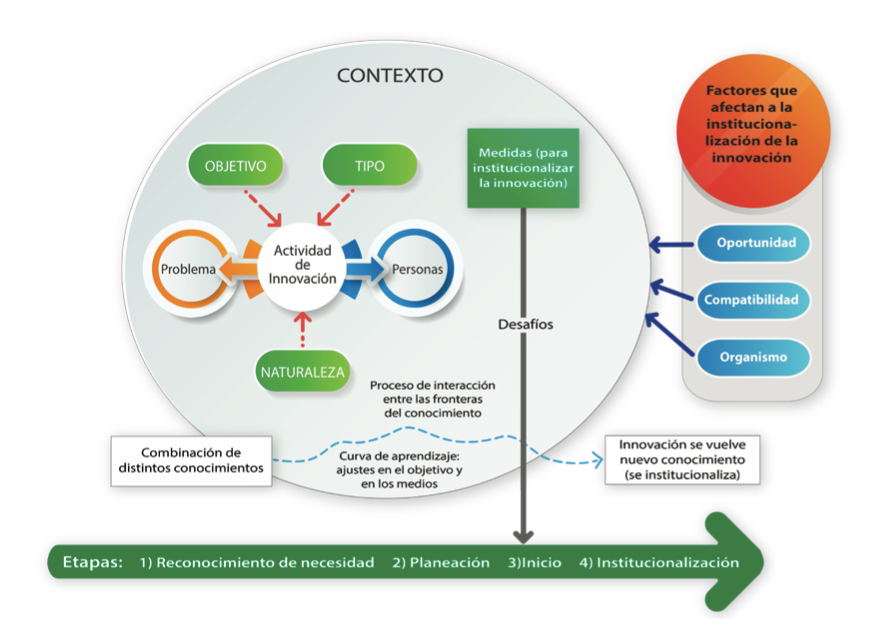
\includegraphics[scale=0.5]{idea_innovacion.png}
    \caption{Segun Sánchez, M. y Escamilla, J.(2018) hace referencia que la intitucionalización del conocimiento debe abarcar actividades de innovación que permitan conjuntar el problema con el sujeto focalizándose en el cumplimiento del objetivo, el tipo y la naturaleza de la innovación, mediante una serie de etapas de forma sistematizada. }
    \label{fig:innovación}
\end{figure}


\subsection{Aporte personal}
Una vez analizado el artículo, me permití tomar el mismo, en específico el apartado de las entrevistas para realizar las siguientes actividades que permitió evaluar las problemáticas constantes referidos en el documento; siguiendo los siguientes pasos:
\begin{enumerate}
    \item Analizar las temáticas para encontrar problemáticas semejantes en cada país, de las cuales se detectó infraestructura, actividades y capacitación.
    \item Se identificaron palabras claves que encajaran en el contexto de la problemática.
    \item Se hizo un filtrado de signos de puntuación en el texto para que no se arroje texto basura.
    \item Se realizó la búsqueda de palabras claves por país analizado, almacenando la frecuencia de éstas en una matriz de 10 x 3, donde en la primer columna se almacena la frecuencia de las palabras claves de infraestructura, en la segunda columna se almacena la frecuencia de las palabras claves de la actividad y en la tercera columna se almacena la frecuencia de las palabras claves de capacitación.
    \item Se sumó todos los valores de la primer columna y se almacenó en un vector de tamaño 3, donde el resultado de ésta se guardó en la primer columna, seguidamente la segunda y tercer columna se realizó el mismo procedimiento, para originar el resultado de frecuencia globales por temática.
    \item Al tener la frecuencia global y la frecuencia por país se utilizó la librería de Matplotlib, para graficar cada una de éstas, dando como resultado las imágenes en gráficas de pastel, mediante el ploteo de las matrices.
    \item Una vez obtenida las gráficas correspondientes se hizo el análisis vertido en las conclusiones.
    \item Una vez de desarrollar el análisis de los pasos previos se creó un documento realizado en la plataforma de Overleaf \citep{Overleaf} y el lenguaje de maquetado LaTeX \citep{latex}, con el fin de tener un documento formal sobre el trabajo realizado.
    \item Finalizado el trabajo se subió al repositorio de GitHub romulotroncosop \citep{Github}.
\end{enumerate}

\section{Conclusiones}
A modo de conclusión y después de realizar un análisis exhaustivo del artículo se puede llegar a las siguientes conclusiones:
\begin{enumerate}
    \item Es indispensable establecer diferencias entre los modelos aplicados e integrados en los diversos países estudiados; como también es importante brindar soluciones a los problemas emergentes de la pandemia COVID-19 como son características de logística-académica, tecnología, pedagogía y áreas socio afectivas.
    \item Es importante establecer un rediseño del proceso de enseñanza-aprendizaje que pueda ser adaptada a los niveles educativos de niveles universitarios.
    \item En la integración de las frecuencias evaluadas mediante el análisis del lenguaje contextual se clasificó en tres temáticas de evaluación, según el artículo evaluado. Las tres temáticas fueron Infraestructura, Actividades y Capacitación.
\end{enumerate}
Con los resultados obtenidos mediante el lenguaje de programación Python \citep{python}, apoyándose en la librería de graficación matplotlib \citep{matplot}, se concluye que:
\begin{enumerate}
    \item En términos de graficación general la de mayor problemas fue la infraestructura (48.1 porciento), seguida de las actividades(37 porciento) y finalizando con la capacitación (14.8 porciento). Por lo que, considerando estos porcentajes existen deficiencias de corte de infraestructura como problema principal; relacionado a las actividades donde se incluye las evaluaciones como parámetro de búsqueda, la deficiencia persiste en la forma de evaluación, tomando como último porcentaje la capacitación tomando como parámetro de búsqueda la adaptación, en virtud, de que algunos ya manejaban sistemas híbridos de educación.
    \item Los países que tuvieron mayores quejas en la infraestructura en orden descendente fueron Venezuela, Ecuador, Colombia, Costa Rica y Chile integrando una porcentualidad de 60 o mayor. Dato que se interpreta como una de las mayores quejas de las universidades analizadas. Por otra parte el área evaluada de actividades las mayores fueron Republica Dominicana, Uruguay , Argentina y México; Dato en el que se concluye la resistencia de pasar de la educación tradicional (educación 3.0) a la digital(educación 4.0).  
\end{enumerate}

\begin{figure}[ht]
    \centering
    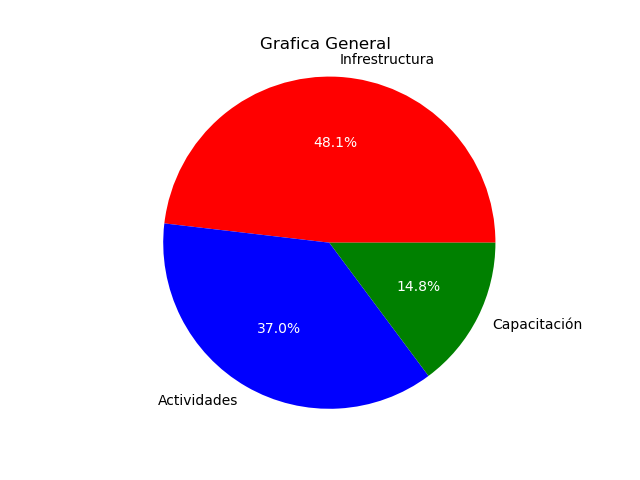
\includegraphics[scale=0.8]{General.png}
    \caption{En la gráfica general se muestra el mayor porcentaje de problemas en los datos obtenidos fue la infraestructura, seguido de las actividades y la capacitación. }
    \label{fig:general}
\end{figure}



\begin{figure}[ht]
    \centering
    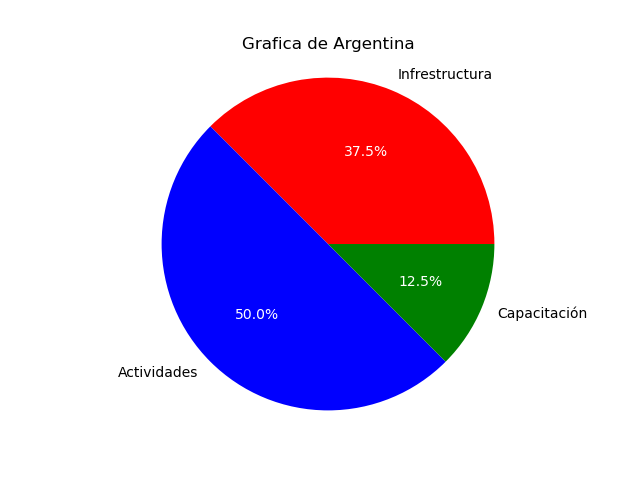
\includegraphics[scale=0.8]{Argentina.png}
    \caption{El país de Argentina, analizado de manera individual, los datos registrados hacen referencia que el mayor problema son las actividades seguidas de la infraestructura y la capacitación.}
    \label{fig:argentina}
\end{figure}

\begin{figure}[ht]
    \centering
    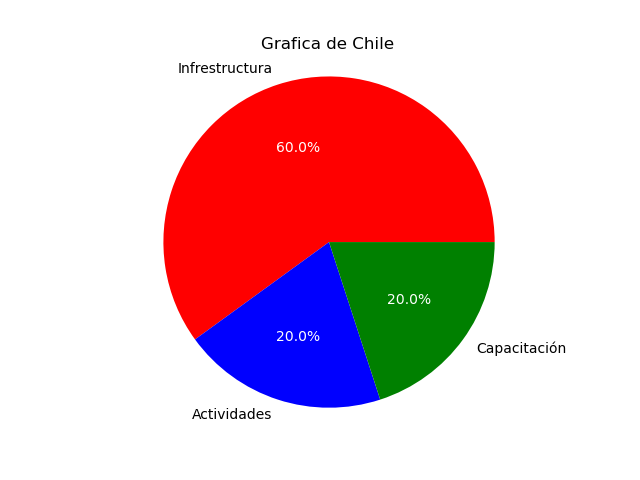
\includegraphics[scale=0.8]{Chile.png}
    \caption{El país de Chile, analizado de manera individual, los datos registrados hacen referencia que el mayor problema es la infraestructura seguidas de las actividades y la capacitación.}
    \label{fig:chile}
\end{figure}

\begin{figure}[ht]
    \centering
    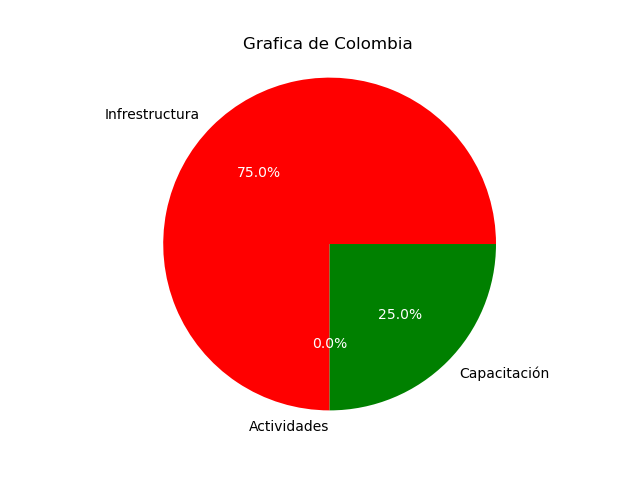
\includegraphics[scale=0.8]{Colombia.png}
    \caption{El país de Colombia, analizado de manera individual, los datos registrados hacen referencia que el mayor problema es la infraestructura seguidas únicamente de la capacitación, omitiendo problemas de actividades.}
    \label{fig:colombia}
\end{figure}

\begin{figure}[ht]
    \centering
    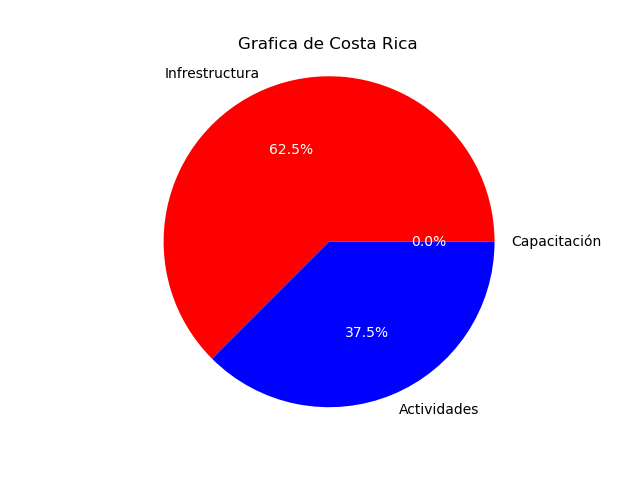
\includegraphics[scale=0.8]{Costa_Rica.png}
    \caption{El país de Costa Rica, analizado de manera individual, los datos registrados hacen referencia que el mayor problema es la infraestructura seguidas únicamente de las actividades, omitiendo problemas de capacitación.}
    \label{fig:costa_rica}
\end{figure}

\begin{figure}[ht]
    \centering
    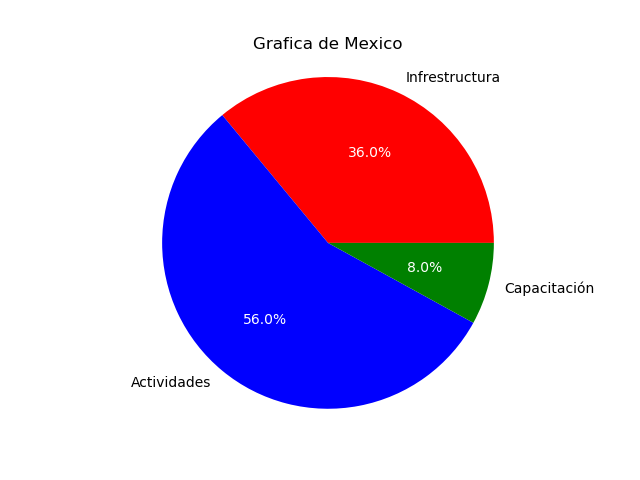
\includegraphics[scale=0.8]{Mexico.png}
    \caption{El país de México, analizado de manera individual, los datos registrados hacen referencia que el mayor problema son las actividades seguidas de la infraestructura y la capacitación.}
    \label{fig:mexico}
\end{figure}

\begin{figure}[ht]
    \centering
    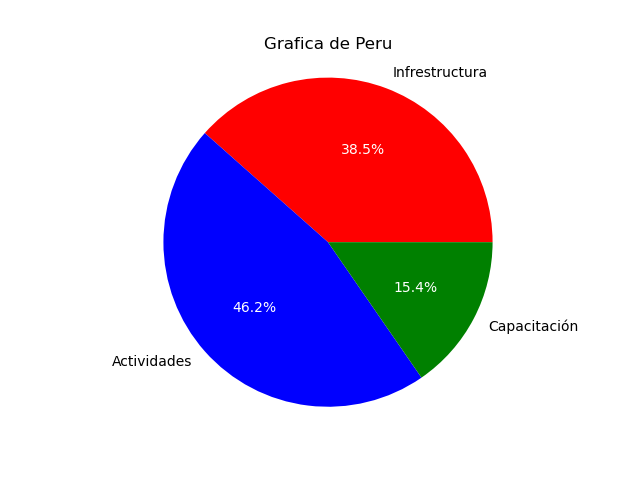
\includegraphics[scale=0.8]{Peru.png}
    \caption{El país de Perú, analizado de manera individual, los datos registrados hacen referencia que el mayor problema es la infraestructura seguidas de las actividades y la capacitación.}
    \label{fig:peru}
\end{figure}

\begin{figure}[ht]
    \centering
    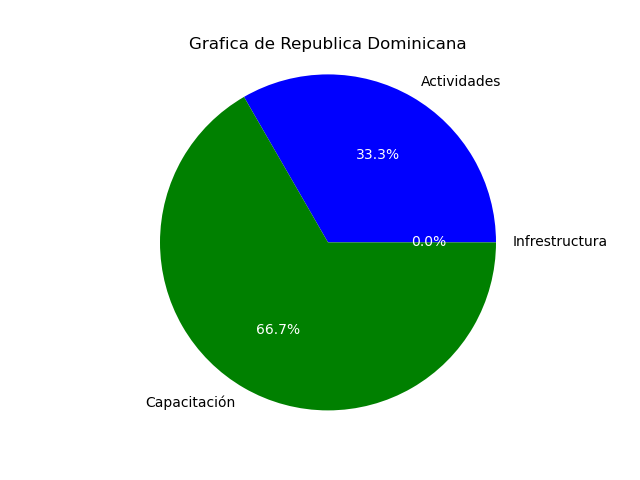
\includegraphics[scale=0.8]{Republica_Dominicana.png}
    \caption{El país República Dominicana, analizado de manera individual, los datos registrados hacen referencia que el mayor problema es la capacitación seguida únicamente de las actividades, omitiendo problemas de infraestructura.}
    \label{fig:costa_rica}
    \label{fig:republica_dominicana}
\end{figure}

\begin{figure}[ht]
    \centering
    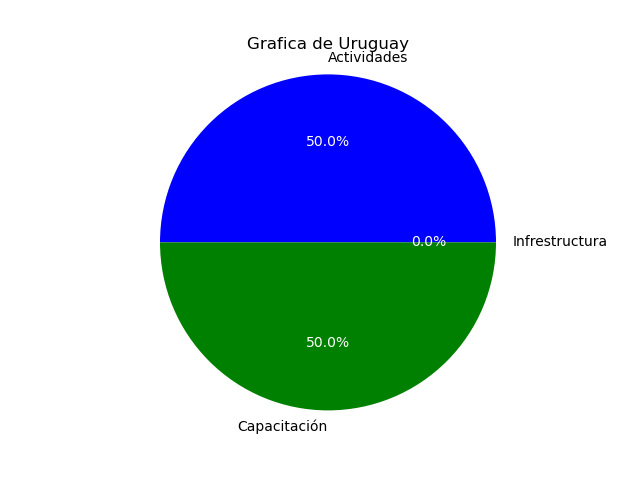
\includegraphics[scale=0.8]{Uruguay.png}
    \caption{La república de Uruguay, analizada de manera individual, los datos registrados hacen referencia que el problema se centra en las actividades y la capacitación, omitiendo problemas de infraestructura.}
    \label{fig:uruguay}
\end{figure}

\begin{figure}[ht]
    \centering
    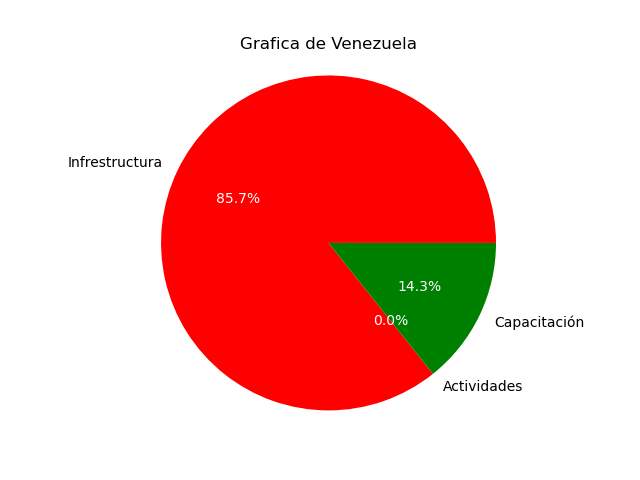
\includegraphics[scale=0.8]{Venezuela.png}
    \caption{El país de Venezuela, analizado de manera individual, los datos registrados hacen referencia que el problema sustancial es la infraestructura seguidas únicamente de la capacitación, omitiendo problemas de actividades.}
    \label{fig:venezuela}
\end{figure}
\clearpage
\bibliographystyle{plain}
\bibliography{references}
\end{document}
